
\chapter{Dinic's Algorithm} \label{dnc}

L'algoritmo segue l'\href{https://en.wikipedia.org/wiki/Edmonds%E2%80%93Karp_algorithm}{Edmonds-Karp} ma ragionando sul fatto che ogni volta che eseguo una BFS creo un albero di copertura con \underline{livelli} che indicano la distanza dal nodo di partenza.
quindi invece di eseguire una BFS e poi saturare solo uno dei percorsi minimi trovati, posso saturarli tutti prima di eseguire di nuovo una BFS.\\
Ogni volta che si esegue una BFS dalla \textit{source} si entra nella \textbf{blocking flow phase}.\\
\begin{definition}{Blocking flow}{}
    Per \textbf{blocking flow} si intende un flusso su un grafo (in questo caso il residuo del level graph) che satura almeno un arco per ogni possibile \textit{path} da $s\rightarrow t$.    
\end{definition}
\begin{obs}{Max flow $\implies$ blocking flow}{}
    Il max flow è un blocking flow ma non è vera l'implicazione opposta.
\end{obs}
per \textbf{level graph} si intende l'albero di copertura dato da una BFS che riporta per ogni nodo la distanza dalla radice, dividendo così il grafo in livelli.
\begin{center}
    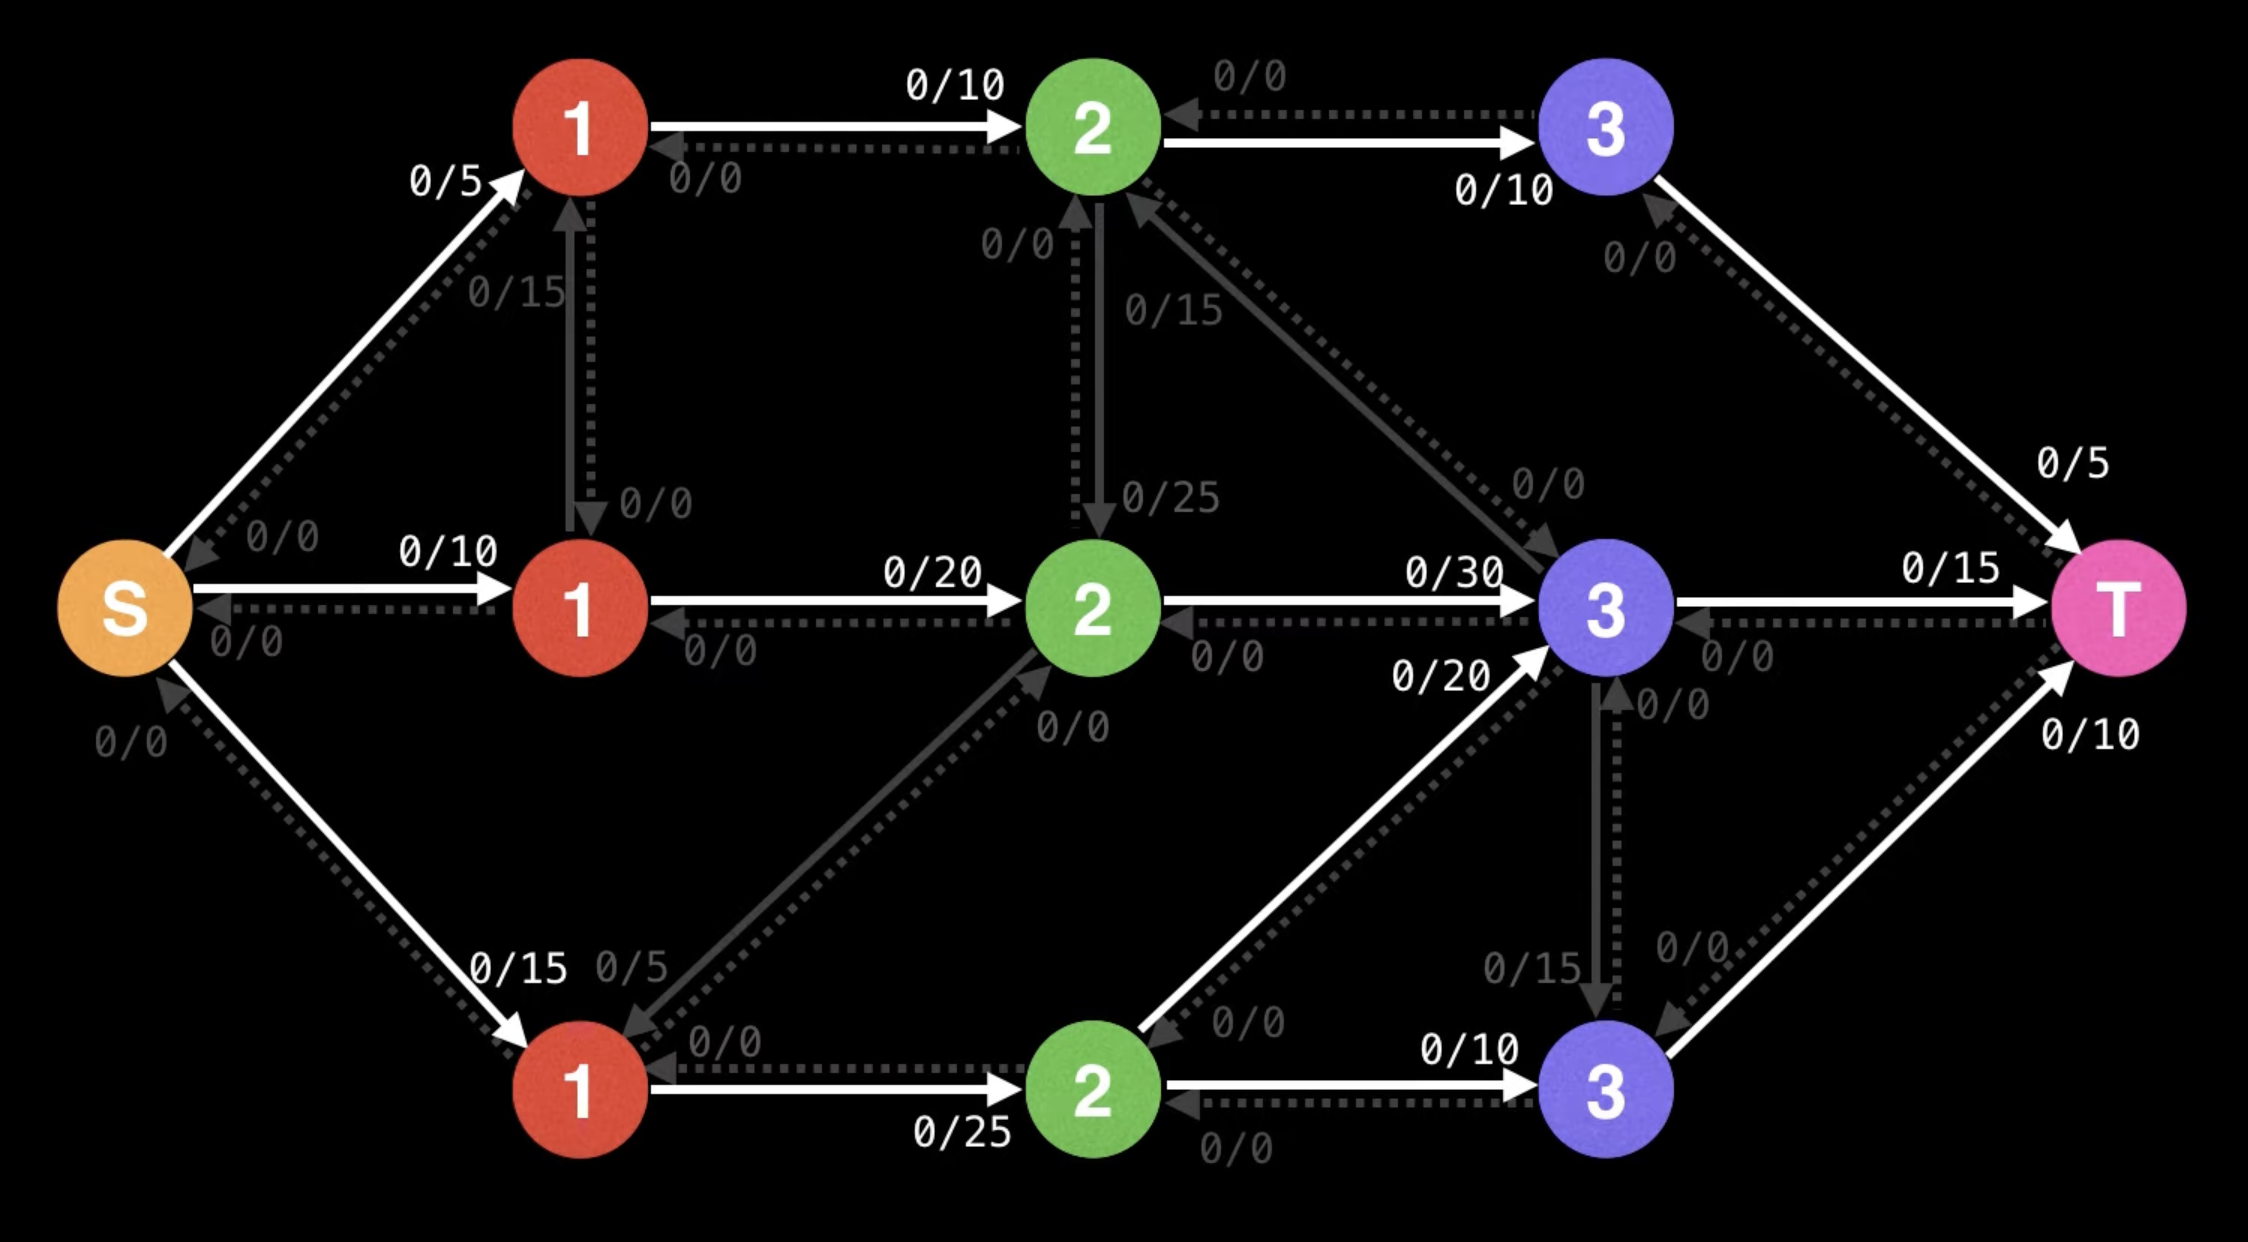
\includegraphics[height=5.25cm]{resources/images/levelGraph.png}\\
    \textit{source: \href{https://www.youtube.com/watch?v=M6cm8UeeziI&t=2s}{Dinic's Algorithm by WilliamFriset}}
\end{center}
In questo modo si riduce il costo dell'algoritmo da $O(n^2m)$ per Edmonds Karp a $O(nm^2)$
\paragraph{Altri link utili}\begin{enumerate}
    \item \href{http://courses.csail.mit.edu/6.854/16/Notes/n10-blocking_flows.html}{Lecture from MIT}
    \item \href{https://en.wikipedia.org/wiki/Dinic%27s_algorithm}{Wikipedia}
\end{enumerate}

\cleardoublepage

